
\begin{frame} \frametitle{Future - Tool Support}
\begin{itemize}
\begin{small}
\item Type-checker
\item Debugging information
%  \begin{itemize}
%  \item Line numbers
%  \item Common programming mistakes
%  \item Mis-spellings (e.g. `Did you mean ...?`)
%  \end{itemize}
\item Automated card \emph{balancer} (e.g. `Maybe card XXX should be \$1 cheaper.`)
\item Develop more complex card examples for reference use
\item Library of AI players using various heuristics
\item Markup language conversion tools / support
\item Graphical (in-browser flash game?) client-server support
\end{small}
\end{itemize}
  \begin{center}
    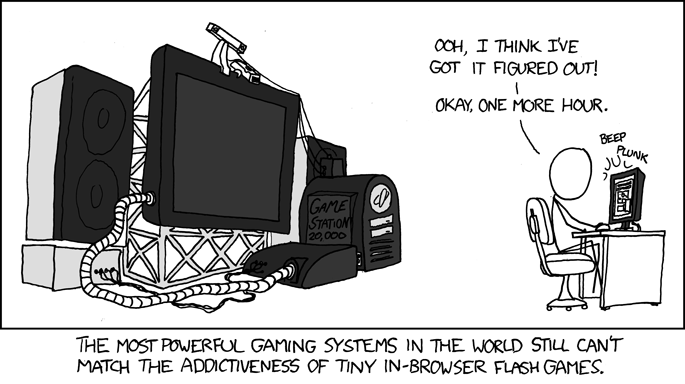
\includegraphics[width=.5\columnwidth]{flash_games.png}
  \end{center}
\footnotetext[1]{
  {\tiny image from \href{https://xkcd.com/484/}{xkcd.com/484}}
}
\end{frame}

\begin{frame} \frametitle{Future - Language Goals}
\begin{itemize}
\item Language support for English-like effect descriptions
\item Card-balancing algorithm
\item Comma-delimited syntactic sugar
\end{itemize}
\end{frame}

